% !TEX root = deckblatt2b.tex

\section{RLC-Tiefpass}
\subsection{Aufgabenstellung}
In diesem Beispiel war ein RLC-Tiefpass aufzubauen und mit drei verschiednen Widerst\"anden jeweils die Sprungantwort und das Bodediagramm zu messen.

\subsection{Schaltung}
\begin{figure}[H]
  \begin{center}
    \begin{circuitikz}[scale=1.3]
      \draw
    (0,0) to[sinusoidal voltage source,v<=$U_1$] (0,2) % The voltage source
          to[L=$1mH$] (3,2)
          to[R=$22\Omega$] (6,2)
          to[C=$100nF$] (6,0)
          to[short] (0,0);
    \end{circuitikz}
    \caption{RLC-Glied Messschaltung.}
  \end{center}
\end{figure}
\noindent
Der Widerstand $R$, wird im laufe der Messungen zweimal ersetzt, einmal durch $180\Omega$ und einmal durch $1k\Omega$. \\ \\
\noindent
Hier handelt es sich um einen Tiefpass zweiter Ordnung, dies ist daran zu erkennen dass, der Schaltkreis zwei frequenzabh\"angige Bauelemente (L und C) enth\"alt. W\"ahrend die Impedanz der Spule im seriellen Zweig mit steigender Frequenz gr\"o\ss{}er wird, so wird die Impedanz des Kondensators im Parallelzweig kleiner. \\
Bei sehr niedrigen Frequenzen (10 - 1000Hz) ist der Blindwiderstand des Kondesantors gr\"o\ss{}er $1500\Omega$, w\"hrend die Spule einen Blindwiderstand von kleiner $1\Omega$ hat. An dem Verh\"altnism\"a\ss{}ig gro\ss{}en Widerstand im Parallelzweig f\"allt daher sehr wenig Spannung ab und der Tiefpass hat eine sehr geringe D\"ampfung. Steigt nun die Frequenz, \"andern sich auch die Blindwiderst\"ande und der Spannungsabfall am Kondensator wird immer gr\"o\ss{}er, was zu einer gr\"o\ss{}eren D\"ampfung f\"uhrt.

\subsection{Sprungantwort $R=22\Omega$}

\begin{figure}[H]
  \begin{center}
    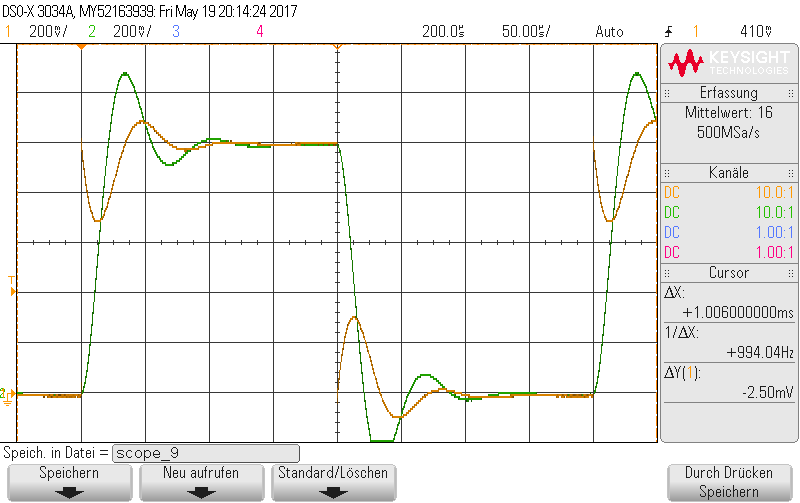
\includegraphics[width=1\textwidth]{./Oszi_Bilder/RLC_Sprung_22.png}
    \caption{Sprungantwort mit $R=22\Omega$}
  \end{center}
\end{figure}
\noindent
Bereits in der Sprungantwort ist zu erkennen, dass das System mit einem Widerstand von nur $22\Omega$ \"uberschwingen wird, da die Ausgangsspannung an den Flaken stark \"uberschwingt. Die Schwingungen an der Eingangsspannung werden durch die Spule in der Schaltung verursacht.

\subsection{Bodediagramm $R=22\Omega$}

\begin{figure}[H]
  \centering
  \begin{tikzpicture}
    \begin{axis}[width=15cm, height=7cm, xmode=log, xmin=10, xmax=1e7, xlabel={$Hz$}, ylabel={dB},y tick label style={grid=major}]
      \addplot table[x=Frequenz, y=dB, col sep=comma] {./csv_files/RLC_22_amplitude.csv};
      %\node[label={260:{$f_g$}},circle,fill=black,inner sep=3pt] at (axis cs:15580,12) {};
    \end{axis}
  \end{tikzpicture}
  \caption{Bode Diagramm RLC-Tiefpass, $R=22\Omega$, Amplitudengang}
\end{figure}
\begin{figure}[H]
  \centering
  \begin{tikzpicture}
    \begin{axis}[width=15cm, height=7cm, xmode=log, xmin=10, xmax=1e7, xlabel={$Hz$}, ylabel={Phase},y tick label style={grid=major}]
      \addplot table[x=Frequenz, y=Phase, col sep=comma] {./csv_files/RLC_22_phase.csv};
      %\node[label={260:{$f_g$}},circle,fill=black,inner sep=3pt] at (axis cs:15580,12) {};
    \end{axis}
  \end{tikzpicture}
  \caption{Bode Diagramm RLC-Tiefpass, $R=22\Omega$, Phasengang}
\end{figure}
\noindent
Da es sich bei dieser Messung um einen Tiefpass handelt is die D\"ampfung bis zur Grenzfrequenz 0dB und das Eingangsignal wird unver\"andert durchgelassen. Wie bereits in der Sprungantwort festgestellt schwingt das Filter genau bei der Grenzfrequenz, das heißt die Ausgangsspannung ist gr\"o\ss{}er als die Eingangspannung. Danach beginnt das Fiter mit $-40dB/Dec$ zu d\"ampfen. Die Phase dreht von $0^\circ$ auf $-180^\circ$, genau bei der Grenzfrequenz ist die Phase auf $-90^\circ$. \\
Die letzten 5 Messpunkte sind sehr ungenau, da das Ausgangssignal bereits so stark ged\"ampft ist, dass keine genauen Messungen mehr durchgef\"uhrt werden konnten. \\ \\
Die genaue Grenzfrequenz sollte mittels Variation der Frequenz festgestellt werden. Die Frequenz am Funktionsgenerator wird so lange erh\"oht bis die Phasenverschiebung genau $-90^\circ$ betr\"agt. \\ \\
Ermittelte Grenzfrequenz: $f_0=15580Hz$ \\ \\
Berechnete Grenzfrequenz: $f_0=\frac{1}{2\pi * \sqrt{LC}}=\frac{1}{2\pi * \sqrt{100nF*1mH}} = 15916Hz$ \\ \\
Unterschied zwischen berechneter/gemessener Werte: $2,11\%$


\subsection{Sprungantwort $R=180\Omega$}

\begin{figure}[H]
  \begin{center}
    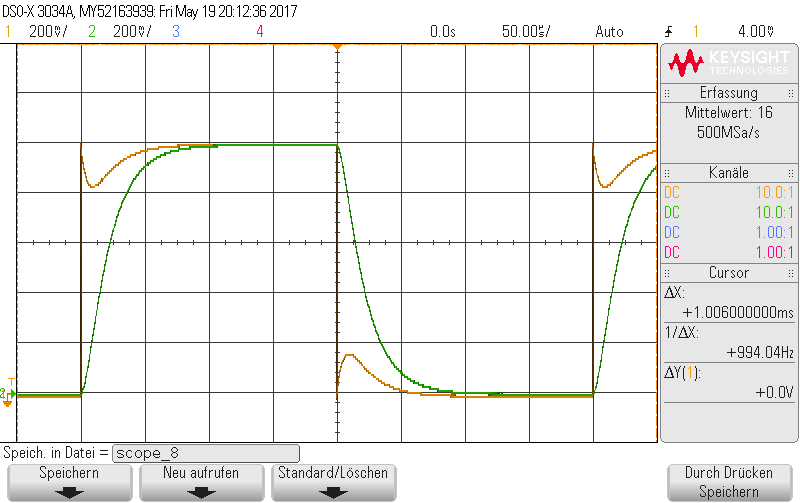
\includegraphics[width=1\textwidth]{./Oszi_Bilder/RLC_Sprung_180.png}
    \caption{Sprungantwort mit $R=180\Omega$}
  \end{center}
\end{figure}
\noindent
Mit dem gr\"o\ss{}eren Widerstand, steigt die Ausgangsspannung reltativ schnell an, es kommt jedoch nicht zu \"uberschwingungen $\Rightarrow$ Filter kritischer D\"ampfung. \\

\subsection{Bodediagramm $R=180\Omega$}

\begin{figure}[H]
  \centering
  \begin{tikzpicture}
    \begin{axis}[width=15cm, height=7cm, xmode=log, xmin=10, xmax=1e7, xlabel={$Hz$}, ylabel={dB},y tick label style={grid=major}]
      \addplot table[x=Frequenz, y=dB, col sep=comma] {./csv_files/RLC_180_amplitude.csv};
      %\node[label={260:{$f_g$}},circle,fill=black,inner sep=3pt] at (axis cs:15580,12) {};
    \end{axis}
  \end{tikzpicture}
  \caption{Bode Diagramm RLC-Tiefpass, $R=180\Omega$, Amplitudengang}
\end{figure}
\begin{figure}[H]
  \centering
  \begin{tikzpicture}
    \begin{axis}[width=15cm, height=7cm, xmode=log, xmin=10, xmax=1e7, xlabel={$Hz$}, ylabel={Phase},y tick label style={grid=major}]
      \addplot table[x=Frequenz, y=Phase, col sep=comma] {./csv_files/RLC_180_phase.csv};
      %\node[label={260:{$f_g$}},circle,fill=black,inner sep=3pt] at (axis cs:15580,12) {};
    \end{axis}
  \end{tikzpicture}
  \caption{Bode Diagramm RLC-Tiefpass, $R=180\Omega$, Phasengang}
\end{figure}
Da es sich hier um ein Filter kritischer D\"ampfung handelt, beginnt die D\"ampfung, kurz vor der Grenzfrequenz. Bei genau $-90^\circ$ Phasenverschiebung, d\"ampft das Filter mit -5dB. Ab der Grenzfrequenz wird mit -40dB/Dec ged\"ampft.

\subsection{Sprungantwort $R=1k\Omega$}

\begin{figure}[H]
  \begin{center}
    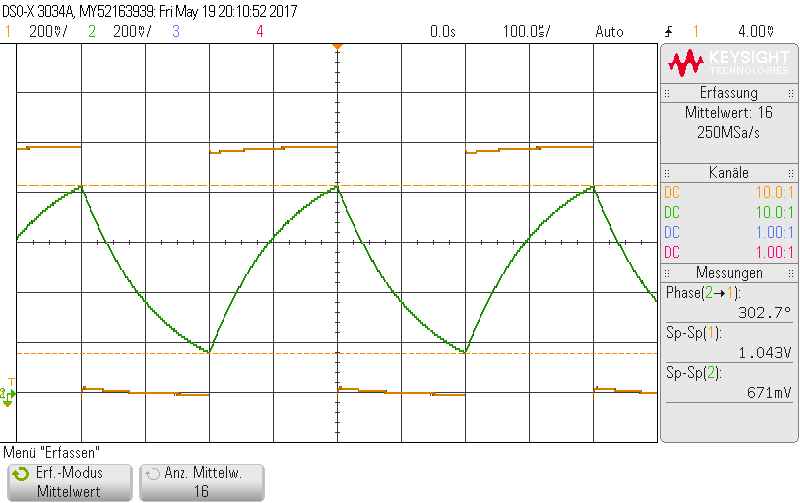
\includegraphics[width=1\textwidth]{./Oszi_Bilder/RLC_Sprung_1k.png}
    \caption{Sprungantwort mit $R=1k\Omega$}
  \end{center}
\end{figure}
\noindent
Mit einem sehr gro\ss{}en Widerstand von $R=1k\Omega$ ist die Zeitkonstante $\tau$ sehr gro\ss{}, d.h. das Filter braucht sehr lange bis die D\"ampfung erreicht wird.

\subsection{Bodediagramm $R=1k\Omega$}

\begin{figure}[H]
  \centering
  \begin{tikzpicture}
    \begin{axis}[width=15cm, height=7cm, xmode=log, xmin=10, xmax=1e7, xlabel={$Hz$}, ylabel={dB},y tick label style={grid=major}]
      \addplot table[x=Frequenz, y=dB, col sep=comma] {./csv_files/RLC_1k_amplitude.csv};
      %\node[label={260:{$f_g$}},circle,fill=black,inner sep=3pt] at (axis cs:15580,12) {};
    \end{axis}
  \end{tikzpicture}
  \caption{Bode Diagramm RLC-Tiefpass, $R=1k\Omega$, Amplitudengang}
\end{figure}
\begin{figure}[H]
  \centering
  \begin{tikzpicture}
    \begin{axis}[width=15cm, height=7cm, xmode=log, xmin=10, xmax=1e7, xlabel={$Hz$}, ylabel={Phase},y tick label style={grid=major}]
      \addplot table[x=Frequenz, y=Phase, col sep=comma] {./csv_files/RLC_1k_phase.csv};
      %\node[label={260:{$f_g$}},circle,fill=black,inner sep=3pt] at (axis cs:15580,12) {};
    \end{axis}
  \end{tikzpicture}
  \caption{Bode Diagramm RLC-Tiefpass, $R=1k\Omega$, Phasengang}
\end{figure}
Dieses schlechte D\"ampfungsverhalten, welches bereits in der Sprunganwort zu erkenne war, zeichnet sich auch im Bodediagramm ab. Das Filter beginnt bereits sehr fr\"uh zu d\"ampfen, jedoch betr\"agt die Filtersteilheit nur -20dB/Dec. Dies liegt daran, dass nur der RC-Teil aktiv ist. Die Grenzfrequenz des RL-Teils liegt weit dar\"uber, bei ca. $150kHz$. Dieser Knick ist allerdings im Amplitudengang nur mehr sehr schlecht zu erkennen, da bei dieser hohen Frequenz das Ausgangsegnal beretis so stark ged\"ampft wrude, dass keine vern\"uftigen Messergebnisse mehr aufgenommen werden konnten. Im Phasengang, ist die Drehung von $-90^\circ$ auf $-180^\circ$ bei ca. $150kHz$ zu erkennen. \\ \\
Grenzfrequenz des RC-Teiles: $f_g=\frac{1}{2\pi RC}=\frac{1}{2\pi*1k\Omega *100nF}=1591Hz$ \\ \\
Grenzfrequenz des LC-Teiles: $f_g=\frac{R}{2\pi L} = \frac{1k\Omega}{2\pi*1mH}=159155Hz$

\subsection{Pol- Nullstellendiagramm}

\subsection{Vergleich: Messung und Simulationen}
Die Messungen stimmen bis auf kleine Bauteil- und Messungenauigkeiten mit den Simulationen \"uberein. \\
Die Messungen von der Ausgangssingale in seine sehr Hochfrequenten Bereich ($>100kHz$) sind im Vergleich zu den Simulationen sehr ungenau, da das Signal bereits zu stark ged\"ampft ist.
